\def\col{blue}
\documentclass[14pt, \col, hyperref={pdfpagelabels=false}]{beamer}
\usepackage[frenchb]{babel} % langue francaise
\usepackage[utf8]{inputenc} % encodage UTF-8
\usepackage[T1]{fontenc} % encodage de la police de caracteres
\usepackage{lmodern}
\usepackage{listings}
\usepackage{multicol}
\usepackage{pifont} %\ding{number}, 
\usepackage{subfigure}
\usepackage{graphicx}
\usepackage{listings}

\usetheme{Warsaw}
\usepackage[\col]{optional} %red blue green
%% THÈMES couleur
%% \usecolortheme{dolphin}
%% \usecolortheme{seahorse}
%% * thèmes globaux : beetle, crane, fly, seagull.
%% * thèmes internes : lily (enlève surtout des couleurs), orchid, rose.
%% * thèmes externes : whale, seahorse, dolphin

% rubber: rules ./rules.ini

 
\mode<presentation>
{
  %%%% Couleurs
  \definecolor{red2}{rgb}{0.8,0.15,0.15}
  \definecolor{bx}{rgb}{0.45,0.05,0.05}  
  \definecolor{ivoire}{rgb}{1, 0.97, 0.9}
 
  \definecolor{bleu2}{rgb}{0.9, 0.90, 1}
  \definecolor{bleu3}{rgb}{0.15,0.15,0.7}
  \definecolor{myblue}{rgb}{0.50,0.55, 0.8}  
  \definecolor{myblue2}{rgb}{0.25,0.3, 0.65}  
  
 \definecolor{mygreen2}{rgb}{0.15,0.60,0.15}
 \definecolor{green2}{rgb}{0.15,0.40,0.15}
  \definecolor{mygreen}{rgb}{0.40,0.7, 0.4}  
%  \definecolor{lightgreen}{rgb}{0.5,0.8, 0.5}  
  \definecolor{lightgreen}{rgb}{0.95, 1, 98}
  
  \definecolor{medium-grey}{gray}{0.45}
  \definecolor{light-grey}{gray}{0.85}
  
  % Couleur des structures et fond dégradé
  % defaut: green
  \setbeamercolor{normal text}{fg=black,bg=lightgreen}
  \setbeamercolor{structure}{fg=green2, bg=light-grey} 
  \setbeamercolor{alerted text}{fg=green2}
  \setbeamertemplate{background canvas}[vertical
    shading][top=lightgreen!100,bottom=lightgreen!30]
  
  \opt{blue}{
    \setbeamercolor{normal text}{fg=black,bg=bleu2}
    \setbeamercolor{structure}{fg=myblue, bg=light-grey} 
    \setbeamercolor{alerted text}{fg=myblue2}
    \setbeamertemplate{background canvas}[vertical
      shading][top=bleu2!100,bottom=bleu2!30]
  }
  \opt{red}{
    \setbeamercolor{normal text}{fg=black,bg=ivoire}
    \setbeamercolor{structure}{fg=bx, bg=light-grey} 
    \setbeamercolor{alerted text}{fg=red2}
    \setbeamertemplate{background canvas}[vertical
      shading][top=ivoire!40,bottom=ivoire!100]
  }
  \opt{green}{
    \definecolor{green2}{rgb}{0.1,0.60,0.1}
    \usecolortheme{dolphin}
  }   
  
  
  \setbeamertemplate{navigation symbols}{}
  \setbeamerfont{title in head/foot}{size=\scriptsize}
  \setbeamerfont{date in head/foot}{size=\scriptsize} 
  
  % Pied de page
  \setbeamertemplate{footline}{
    \hbox{%
      \begin{beamercolorbox}[wd=.4\paperwidth,ht=3ex,dp=1ex,center]{title in head/foot}
        \usebeamerfont{title in head/foot}\enseignement\hspace{1cm} %\shorttitle
      \end{beamercolorbox}%
      \begin{beamercolorbox}[wd=.5\paperwidth,ht=3ex,dp=1ex,left]{date in head/foot}%
        \usebeamerfont{title in head/foot} 
        \hspace*{1ex} 
        \insertshorttitle
      \end{beamercolorbox}% 
      \begin{beamercolorbox}[wd=.1\paperwidth,ht=3ex,dp=1ex,left]{date in head/foot}%
        \usebeamerfont{date in head/foot} 
        \insertframenumber{} / \inserttotalframenumber%\hspace*{2ex} 
    \end{beamercolorbox}}%
    \vskip0pt%
  }

    % Haut de page
  \setbeamertemplate{headline}{%
    \leavevmode
    \begin{beamercolorbox}[wd=.5\paperwidth,ht=3ex,dp=1.125ex,leftskip=.3cm
        plus1fill,rightskip=.3cm]{section in head/foot}%
      \scriptsize{\insertsection}
    \end{beamercolorbox}%
    \begin{beamercolorbox}[wd=.5\paperwidth,ht=3ex,dp=1.125ex,leftskip=.3cm,rightskip=.3cm
        plus1fil]{subsection in head/foot}%
      \scriptsize{\insertsubsection}
    \end{beamercolorbox}%
  }
  \addtobeamertemplate{headline}{}{%
    \vskip-0.1pt
    \pgfuseshading{beamer@topshade}
    \vskip-2pt}
   %% \let\Tiny=\tiny
  %% \let\TINY=\tiny
}

%% Annonce de plan a chaque transition.
%% \AtBeginSection[]{
%%   \begin{frame}<beamer>
%%     \frametitle{Plan}
%%     \tableofcontents[currentsection,currentsubsection]
%%   \end{frame}
%% }



\newcommand{\bashlisting}[0]{\scriptsize\lstset{language=bash,numbers=left,numberstyle=\tiny,
    xrightmargin=1mm, xleftmargin=1mm, keywordstyle=\color{green2}, %
    keywordstyle[1]=\color{blue}, %
    keywordstyle[2]=\color{yellow}, %
    keywordstyle[3]=\color{red2}}}

\newcommand{\filelisting}[0]{\small\lstset{language=,numbers=left,numberstyle=\tiny,
    xrightmargin=4mm, xleftmargin=6mm, frame=single}}

\definecolor{orange}{rgb}{0.9,0.6,0.4}

\newcommand{\clisting}[0]{\scriptsize
  \lstset{language=c, 
    inputencoding=utf8,
    %identifierstyle=\color{blue},%
    keywordstyle=\color{green2}, %
    keywordstyle[1]=\color{blue}, %
    keywordstyle[2]=\color{yellow}, %
    keywordstyle[3]=\color{red2}, %
    stringstyle=\color{orange}, %
    commentstyle=\color{red2}, %
    numbers=left,
    numberstyle=\tiny,
    xleftmargin=1mm,
    breaklines=true,
}}



\newcommand{\cmd}[1]{\texttt{\footnotesize\textcolor{medium-grey}{#1}}}

\newcommand{\cmdlist}[1]{
  \begin{semiverbatim}\begin{minipage}{\linewidth}  
      \footnotesize\textcolor{medium-grey}{#1}\end{minipage}
\end{semiverbatim}}


\newcommand{\coeur}{c\oe ur\xspace}
\newcommand{\oeuvre}{\oe uvre\xspace}
\newcommand{\coeurs}{c\oe urs\xspace}
\newcommand{\mc}{multic\oe ur\xspace}
\newcommand{\mcs}{multic\oe urs\xspace}

\usepackage{multicol}

%%%%%%%%%%%%%
\def\enseignement{ASR2 Système}
\title[]{\enseignement\\
Système de Fichier}
\author{Stéphanie Moreaud}
\institute{Département d'informatique\\
  IUT Bordeaux 1}
\date{}

%%%%%%%%%%%% 
   
\newcommand{\TITRE}[1]{
  \begin{frame} \begin{center}\huge{#1}\end{center}
\end{frame}
}
\newcommand{\FIGURE}[2]{
  \begin{frame} \frametitle{\insertsubsection} 
    \begin{figure} \includegraphics[width=0.8\linewidth]{fichiers-images/#1} 
    \end{figure} 
    \begin{center}\large{#2}\end{center}
\end{frame} }

%%%%%%%%%%%%%%%%%%%%%%%%%%%%%%%%%%%%%
\begin{document}
\begin{frame}
  \titlepage
\end{frame}

\begin{frame}<beamer>
  \frametitle{Plan} 
      \tableofcontents[sections={1-5},currentsection, hideothersubsections] 
\end{frame}
%Annonce de plan a chaque transition.
\AtBeginSection[]{
  \begin{frame}<beamer> \frametitle{Plan}
    \tableofcontents[currentsection, hideothersubsections] 
  \end{frame}
}

\begin{frame}
\frametitle{Bibliographie}
\bibliographystyle{fr-plain}
\small
\nocite{*}    
\bibliography{bib} 
\vspace{0.5cm}    
D'après les transparents de Michel Billaud.\\
\url{http://www.labri.fr/perso/billaud/}
\end{frame}
%%%%%%%%%%%%%%%%%%%%%%%%%
%%%%%% Let's go!  %%%%%%
%%%%%%%%%%%%%%%%%%%%%%%%%


\section{Fichiers et système de fichiers}
\begin{frame}
  \frametitle{Fichiers}
  Sauvegarde (pérenne) de l'information sous forme de \alert{fichiers}
\begin{itemize}
\item lot d'informations portant un nom, 
\item le plus souvent concervés en mémoire de masse
\end{itemize}

\ding{212} un \alert{contenu} \\
\ding{212} des \alert{méta-données} (attributs du fichier) \\
\begin{itemize}
\item taille
\item propriétaire
\item droits d'accès
\item date de création
\item date de dernier accès
\item ...
\end{itemize}
\end{frame}

\begin{frame}
\frametitle{Fichiers}
\vspace{0.5cm}
Les fichiers sont classés dans des \structure{répertoires}
\begin{itemize}
\item chaque répertoire peut contenir d'autres répertoires
\end{itemize}
\vspace{0.5cm}
\ding{212} organisation arborescente\\
\ding{212} \alert{structure de données} appelée \alert{système de fichiers}.
\end{frame}

\begin{frame}
\frametitle{Système de fichiers}
\vspace{-0.4cm}
\begin{figure}
  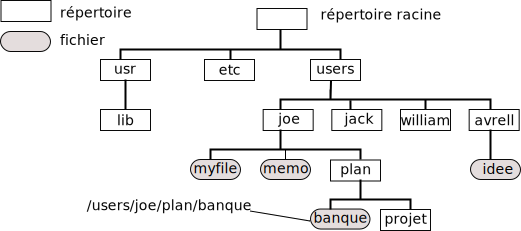
\includegraphics[width=\linewidth]{fig3/file_sys}
\end{figure}
Pour l'utilisateur~: arborescence\\
Fichiers/répertoires accessibles par leur nom\\\ding{212} \alert{chemin d'accès}
\end{frame}


\subsubsection{Système de Gestion de Fichiers}
\begin{frame}
\frametitle{Système de Gestion de Fichiers}
Fonction~: gestion des structures de fichiers 
\begin{itemize}\item Manipulation des fichiers : création, destruction, etc... 
\item Allocation sur la mémoire secondaire 
\item Localisation des fichiers : accès au contenu
\item Sécurité et contrôle des fichiers
\item Fiabilité en cas de panne
\item ...
\end{itemize}
\end{frame}

\section{Organisation du système de fichiers}
\begin{frame}
  \frametitle{\insertsection}
  Fichier = unité d'information abstraite\\
  \vspace{0.5cm}
  Organisation des données varie selon les systèmes de fichiers\\
  \begin{itemize}
  \item allocation disques sur des \alert{blocs} de données 
  \item[\ding{212}] choix des blocs qui composent chaque fichier 
  \end{itemize}
  \vspace{0.5cm}
  Quelques repésentations possibles
  \begin{itemize}
  \item catalogues de fichiers
  \item tables d'allocation (FAT) 
  \item tables de blocs 
  \end{itemize}
\end{frame}

\subsection{Allocation contiguë}
\begin{frame}
  \frametitle{\insertsubsection}
  Stockage de chaque fichier dans une \alert{suite de blocs consécutifs}.\\
  \vspace{0.5cm}
  \underline{Exemple}: Allocation d'un fichier de 24~Ko
  \begin{itemize}
  \item taille des blocs sur le disque = 2~Ko  
  \item[\ding{212}] utilisation de 12 blocs consécutifs. 
  \end{itemize}
  
  \begin{figure}[h]
    \center
    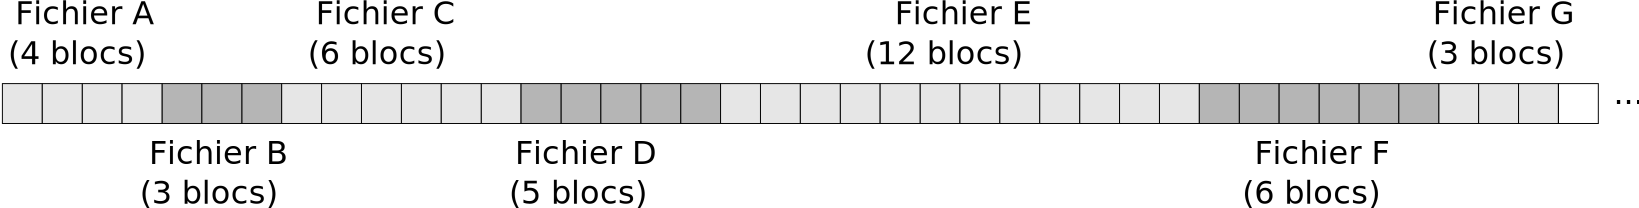
\includegraphics[width=\linewidth]{fig4/alloc_contigue}
  \end{figure}
  \vspace{0.5cm}
\end{frame}

\begin{frame}
  \frametitle{Catalogue de fichiers}
  Mise en \oe{}uvre~: \alert{catalogue de fichiers}
  \vspace{0.5cm}

  Exp~: VTOC = Volume Table of Contents (IBM)
  \begin{itemize}
  \item pas de répertoires, 
  \item fichiers composés de blocs contigus, 
  \item fichiers alloués les uns à la suite des autres sur le disque
  \end{itemize}
\end{frame}

\begin{frame}
  \frametitle{Catalogue de fichiers}
  Au début du disque, une \alert{table de fichier} qui indique
  \begin{itemize} 
  \item le \alert{nom} de chaque fichier
  \item son emplacement (\alert{position premier bloc, taille})
  \end{itemize}
  
  \begin{center}
    \begin{tabular}{|lll|}
      \hline
      \alert{nom} du     & position du & \\
      fichier & \alert{premier bloc} & \alert{taille} \\
      \hline
      CLIENTS & 10 & 50 \\ PRODUITS & 60 & 500 \\ FACTURES & 560 & 2000 \\ ... & ... &
      ... \\
      \hline
    \end{tabular}
  \end{center}
\end{frame}


\begin{frame}
\frametitle{Catalogue de fichiers}
Dans le catalogue~: 
\begin{itemize}
\item table des fichiers
\item liste des \alert{espaces libres}
\end{itemize}
\vspace{0.5cm}

Reste du disque~: contenu des fichiers
\begin{itemize}
\item blocs de données du premier fichier, 
\item puis blocs du second, 
\item etc...
\end{itemize}
\end{frame}
\begin{frame}

\frametitle{VTOC~: occupation du disque}
\begin{figure}
  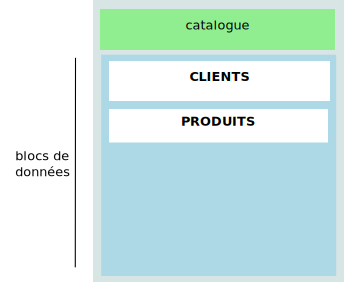
\includegraphics[width=0.8\linewidth]{fig4/vtoc}
\end{figure}
\end{frame}

\begin{frame}
\frametitle{Gestion de l'espace}
\alert{Espaces contigus}
\begin{itemize}
\item \alert{Réservation} d'espace à la création d'un fichier  
\item \alert{Restitution} quand le fichier est supprimé
\item \alert{Extension} des fichiers ?
\end{itemize}
\end{frame}

\begin{frame}
  \frametitle{Avantages/Inconvénients}
  \underline{Avantages}
  \begin{itemize}
  \item simplicité
    \begin{itemize}
    \item information nécessaire~: adresse premier bloc, nb de blocs
    \end{itemize}
  \item performances
    \begin{itemize}
    \item déplacements de bras minimisés
    \end{itemize}
  \end{itemize}
  
  \underline{Inconvénients}
  \begin{itemize}
  \item perte de place
    \begin{itemize}
    \item réservations non utilisées
    \end{itemize}
  \item espaces contigus de taille variable \ding{212} fragmentation
  \end{itemize}
\end{frame}


\begin{frame}
\frametitle{Solutions}
Allocation dans plusieurs zones
\begin{itemize}
\item 1 fichier = plusieurs zones
\item allouées au besoin (dynamiquement)
\end{itemize}
\underline{Exemple}:
réservation d'un fichier de 20 Ko + 5 \alert{extensions} de 10 Ko\\
\vspace{0.5cm}
Utilitaire de réorganisation du disque\\
\vspace{0.5cm}

\underline{Remarque}: allocation contiguë adaptée à d'autres média
\begin{itemize}
\item CD-ROM
\end{itemize}
\end{frame}

\subsection{Allocation par liste chaînée}
\begin{frame}
\frametitle{\insertsubsection}
Fichiers concervés sous forme d'une liste chaînée de blocs disque
\begin{itemize}
\item premier mot de chaque bloc = pointeur sur le bloc suivant
\end{itemize}
\begin{figure}
  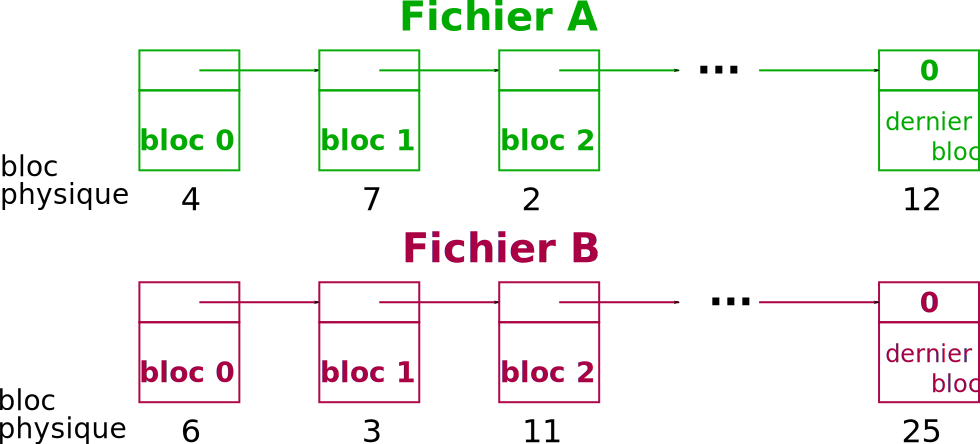
\includegraphics[width=0.8\linewidth]{fig4/liste_chainee}
\end{figure}
\end{frame}

\begin{frame}
  \frametitle{\insertsubsection}
  Fichiers non contigus
  \begin{itemize}
  \item entrée du catalogue contient adresse du premier bloc
  \item extention facile à gérer
  \item pas de perte d'espace 
  \end{itemize}
  \vspace{0.5cm}
  \begin{itemize}
  \item taille des données d'un bloc = puissance de 2 - taille pointeur
  \item parcours séquentiel des blocs \ding{212} multiples accès aléatoires sur le disque
  \end{itemize}
  \underline{Solution}: utilisation d'une \alert{table d'allocation}
\end{frame}

\begin{frame}
  \frametitle{Table d'allocation}
  Table contenant la position du bloc suivant
  \begin{figure}
    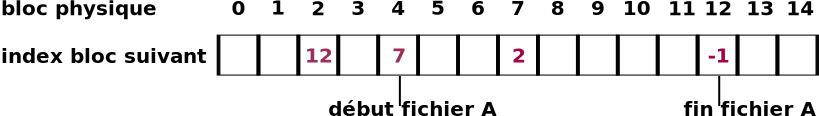
\includegraphics[width=\linewidth]{fig4/table_alloc}
  \end{figure}
\begin{itemize}
\item Pas de pointeurs au début des blocs
\item Table chargée en mémoire principale
  \begin{itemize}
  \item parcours de la table avant tout accès disque  
  \item inconvénient~: espace mémoire occupé par la table
    \begin{itemize}
    \item exp: disque de 200~Go, blocs de 1~Ko\\
      \hspace{0.7cm} \ding{212} 200 millions d'entrées
    \end{itemize}
  \end{itemize}
\end{itemize}
\ding{212} Système \alert{FAT} (\emph{File Allocation Table})  
\end{frame}

\begin{frame}
  \frametitle{Catalogue de fichiers}
  \begin{itemize}
  \item Table des fichiers
    \begin{center}
      \begin{tabular}{|lll|}
        \hline
        \alert{nom} du     & position du & \\
        fichier & \alert{premier bloc} & \alert{taille} \\
        \hline
        CLIENTS & 10 & 50 \\ PRODUITS & 12 & 500 \\ FACTURES & 15 & 2000 \\ ... & ... &
        ... \\
        \hline
      \end{tabular}
    \end{center}
    
  \item \alert{Table de chaînage} des blocs 
    \begin{center}
      \begin{tabular}{|c|c|c|c|c|c|c|}
        \multicolumn{1}{c}{} & \multicolumn{1}{c}{...} & \multicolumn{1}{c}{10} &
        \multicolumn{1}{c}{11} & \multicolumn{1}{c}{12} & \multicolumn{1}{c}{13} &
        \multicolumn{1}{c}{...}\\
        \cline{1-7}
        \small{\alert{bloc suivant}} & ... & 11 & 20 & 13 & 14 & ... \\
        \cline{1-7}% \hline
\end{tabular}
\end{center}
\item puis blocs de données
\end{itemize}
\end{frame}

\begin{frame}
  \frametitle{FAT: occupation du disque}
  \begin{figure}
    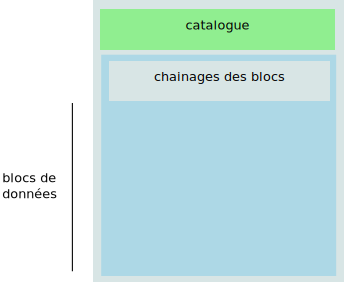
\includegraphics[width=0.8\linewidth]{fig4/fat}
  \end{figure}
\end{frame}

\begin{frame}
\frametitle{Autre représentation}
\alert{Table des blocs} intégrée dans le catalogue

\begin{tabular}{|l|l|cccccc|}
\hline
nom & taille & B1 & B2 & B3 & B4 & .... &B16 \\
\hline
CLIENTS & 3 & 10 & 11 & 22 & - & & -\\ PRODUITS & 4 & 20 & 11 & 42 & - & & -\\
...&&&&&&& \\ FACTURES & 20 & 101 & 102 & 103 & 104 & ... & 116 \\ ...&&&&&&& \\
FACTURES & - & 117 & 118 & 119 & 120 & ... & - \\ ...&&&&&&& \\
\hline
\end{tabular}
\ding{212} utilisation de ``lignes de continuation''\\
\vspace{0.5cm}
Représentation utilisée dans CP/M
\end{frame}

\subsection{Tables des blocs Unix}

\begin{frame}
\frametitle{Utilisation de n\oe{}uds d'index (UNIX)}

A chaque fichier est associé une \alert{structure de données} appellée
\alert{\emph{i-node}} (index-node) qui contient~:
\begin{itemize}
\item les attributs (taille, propriétaire, droits...)
\item les adresses de ses premiers blocs de données
\pause
\item l'adresse d'un \alert{bloc d'indirection simple} 
\begin{itemize}
\item contient d'autres adresses de \textbf{blocs de données}
\end{itemize}
\pause
\item l'adresse d'un \alert{bloc d'indirection double}
\begin{itemize}
\item contient des adresses de \textbf{blocs d'indirection simple}
\end{itemize}
\pause
\item l'adresse d'un \alert{bloc d'indirection triple}
\begin{itemize}
\item contient des adresses de \textbf{blocs d'indirection double}
\end{itemize}
\end{itemize}
\end{frame}

\begin{frame}
  \frametitle{I-nodes et blocs d'indirection}
  \begin{figure}
    \includegraphics[width=0.9\linewidth]{fig4/inode1}
  \end{figure}
\end{frame}
\begin{frame}
  \frametitle{I-nodes et blocs d'indirection}
  \begin{figure}
    \includegraphics[width=0.9\linewidth]{fig4/inode2}
  \end{figure}
\end{frame}
\begin{frame}
  \frametitle{I-nodes et blocs d'indirection}
  \begin{figure}
    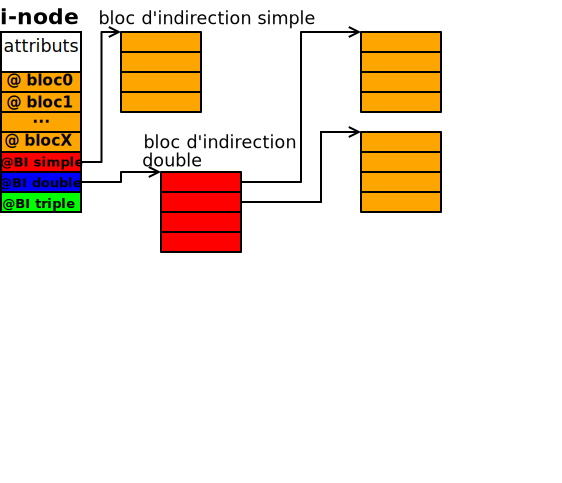
\includegraphics[width=0.9\linewidth]{fig4/inode3}
  \end{figure}
\end{frame}
\begin{frame}
  \frametitle{I-nodes et blocs d'indirection}
  \begin{figure}
    \includegraphics[width=0.9\linewidth]{fig4/inode}
  \end{figure}
\end{frame}

\begin{frame}
\frametitle{Chiffrage}

\structure{Supposons :}
\begin{itemize}
\item des blocs de 4 Ko ($2^{12}$)
\item des adresses sur 32 bits
\end{itemize}

\structure{Capacité maximale du disque} ?
\pause

Avec 32~bits on peut adresser $$ 2^{32} ~\mbox{blocs}$$
\pause
le disque peut ainsi contenir \emph{en théorie} 
$$ 2^{32} \times 2^{12} = 2^{44} ~\mbox{octets} = 16 ~\mbox{Tera octets}$$
\pause
\structure{Question} : taille maximum d'un fichier ?

\end{frame}

\begin{frame}
\frametitle{Taille maximum d'un fichier}
\begin{itemize}
\item une adresse = 32 bits = 4 octets 
\item un bloc = 4 Ko \\\pause \ding{212} peut contenir $4096 = 1024$ adresses.
\end{itemize}
\pause
Donc
\begin{itemize}
\item un \alert{bloc d'indirection simple} conduit à 1024 blocs de données
\pause soit $ 1024 \times 4 \mbox{Ko} $ soit 4 Mo de données
\pause
\item un \alert{BI doubles} conduit à 1024 BI simple (4 Go)
\item un \alert{BI triple} conduit à 1024 BI double (4 To)
\end{itemize}
\ding{212} Pour la plupart des accès, une indirection suffit
\end{frame}


\begin{frame}
\frametitle{Bilan}
\structure{Fichiers contigus} :
\begin{itemize}
\item temps d'accès : très bonne performances
\item problème de gestion des espaces libres
\item convient très bien à des supports en lecture seulement (CD, DVD)
\end{itemize}

\structure{Blocs chainés, table des blocs, i-nodes}
\begin{itemize}
\item gestion souple et efficace de l'espace
\item problèmes de performance si les données sont dispersées
\end{itemize}
\end{frame}


\section{Représentation des répertoires}
\subsection{Comme des catalogues de fichiers}
\begin{frame}
  \frametitle{Comment représenter les arborescences~?}
  
  \ding{212} Comme des catalogues de fichiers
  \begin{itemize}
  \item catalogue arborescent, 
  \item entrées spéciales dans la table des fichiers
  \end{itemize}
  \begin{figure}
    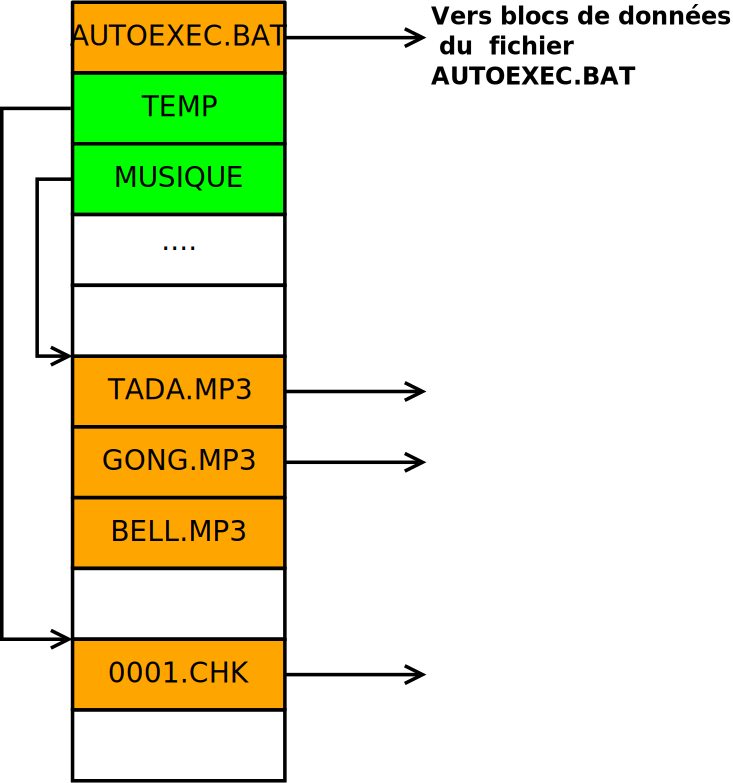
\includegraphics[width=0.4\linewidth]{fig4/repertoires}
  \end{figure}
\end{frame}

\begin{frame}
  \frametitle{Catalogues de fichiers}
  Répertoires matérialisés dans le catalogue par des lignes spéciales qui
  renvoient vers d'autres lignes
  \begin{itemize}
  \item ne permet pas d'avoir des liens, seulement des \emph{raccourcis}
  \item solution adoptée par CP/M, MS/DOS, Windows...
  \end{itemize}
  
  \begin{tabular}{|ll|}
    \hline
    \alert{types de ligne} & information\\
    \hline \hline 
    fichier & taille, blocs \\ \hline vide & \\ \hline répertoire & numéro de
    ligne \\ \hline raccourci & chemin destination \\ \hline
  \end{tabular}
\end{frame}

\subsection{Comme des fichiers de données}
\begin{frame}
  \frametitle{\insertsection}
  \ding{212} Comme des fichiers de données\\
  \vspace{0.5cm}
  Solution utilisée sous Unix\\
  \vspace{0.5cm}
  
  Un système de fichiers contient
  \begin{itemize}
  \item une \alert{table d'\emph{i-nodes}} (noeuds d'information)
  \item des \alert{blocs de données} liés à ces i-nodes
  \end{itemize}
  
  Un fichier/répertoire est identifié par son numéro d'i-node
\end{frame}


\begin{frame}
  \frametitle{Différents types d'i-nodes}
  
  \begin{tabular}{|l|l|}
    \hline 
    types & donnée \\
    \hline
    fichiers & Blocs = contenu du fichier \\ 
    répertoires & Blocs = table de noms, \no i-node \\
    liens symboliques & chemin d'accès \\ périphériques & type,
    majeur, mineur \\ ... & \\
    \hline
  \end{tabular}
\end{frame}

\subsubsection{Exemple}
\begin{frame}
  \frametitle{Exemple d'arborescence}
  \begin{figure}
    \includegraphics[width=0.8\linewidth]{fig4/fichiers-unix}
  \end{figure}
\end{frame}

\begin{frame}
  \frametitle{Table des inodes}
  \begin{figure}
    \includegraphics[width=0.5\linewidth]{fig4/fichiers-unix}
  \end{figure}
  \begin{tabular}{|rcc|l|}
    \hline
    \No & type & CR & contenu des blocs \\
    \hline
    1 & d & 4 & ..=1, .=1, A=2, B=3, C=4 \\ 
    2 & d & 2 & ..=1, .=2, D=5, E=6 \\ 
    3 & f & 1 & ``coucou'' \\ 
    4 & d & 2 & ..=1, .=4, F=7 \\
    % 5 & f & 1 & ``hello, world'' \\
    & & \ldots & \\
    \hline
  \end{tabular}\\
  CR = compteur de références
\end{frame}

\begin{frame}
  \frametitle{Compteur de référence}
  Indique combien de fois l'objet est référencé\\
  CR = 0, on peut récupérer l'espace qu'il occupe.
  
  \begin{multicols}{2}  Après \texttt{ln /B /C/G}
    \begin{figure}
      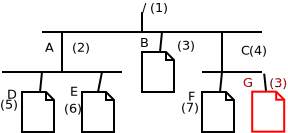
\includegraphics[width=0.9\linewidth]{fig4/fichiers-unix2}
    \end{figure}  
  \end{multicols}
  \small
  \begin{tabular}{|rcc|l|}
    \hline
    \No & type & CR & contenu des blocs \\
    \hline
    1 & d & 4 & ..=1, .=1, A=2, B=3, C=4 \\
     2 & d & 2 & ..=1, .=2, D= 5, E=6 \\ 
     3 & f & \alert{2} & ``coucou'' \\ 
     4 & d & 2 & ..=1, .=4, F=7, \alert{G=3} \\
    % 5 & f & 1 & ``hello, world''\\
    & & \ldots & \\
    \hline
  \end{tabular}
  \normalsize
\end{frame}


\subsection{Gestion des blocs libres}
\begin{frame}
  \frametitle{Gestion des blocs libres}
  Le système possède
  \begin{itemize}
  \item{une liste des \alert{blocs libres}}
  \item{un \alert{tableau de marquage des blocs occupés}}
  \end{itemize}
\end{frame}

\subsubsection{Vérification du système de fichiers}
\begin{frame}
  \frametitle{Vérification du système de fichiers}
  Utilitaire \texttt{fsck}, descente de l'arborescence :
  
  \begin{enumerate}
  \item vérification des i-noeuds, des blocs et des tailles
  \item vérification de la structure des répertoires
  \item vérification de la connectivité des répertoires
  \item vérification des compteurs de référence
  \item vérification de l'information du sommaire de groupe
  \end{enumerate}
  \ding{212} peut être très long.
\end{frame}

\begin{frame}
  \frametitle{Vérification du système de fichiers}
  Vérification des i-noeuds, des blocs et des tailles
  \begin{itemize}
  \item i-noeuds non-détruits $\Rightarrow$ blocs alloués.
  \item blocs alloués $\Rightarrow$ i-noeud.
  \end{itemize}
  Vérification de la structure des répertoires
    \begin{itemize}
    \item numéro d'i-noeud cité dans un répertoire $\Rightarrow$
      i-noeud existant
    \end{itemize}
    Vérification de la connectivité des répertoires
      \begin{itemize}
      \item i-noeuds actifs $\Leftrightarrow$ accessibles depuis la racine
      \end{itemize}
      Vérification des compteurs de référence
      \begin{itemize}
      \item Nombre de références recalculé = nombre de références indiqué dans l'i-noeud
      \end{itemize}
\end{frame}

\section{Autres caractéristiques}
\subsubsection{Journalisation}
\begin{frame}
  \frametitle{Autres caractéristiques~: Journalisation}

  \alert{Systèmes de fichiers journalisés}, \alert{journal} : 
  \begin{itemize} 
  \item garde une trace des opérations d'écriture non terminées
  \item permet de les reprendre en cas d'arrêt brutal
  \end{itemize}
  \vspace{0.5cm}

  \begin{itemize}
  \item[\ding{212}] Pas de pertes d'informations
  \item[\ding{212}] reprise sur incidents plus rapide (évite le \emph{fsck})
  \end{itemize}
\end{frame}


\subsubsection{Snapshots (clichés)}
\begin{frame}
  \frametitle{Snapshots (clichés)}

  Pendant la durée d'une sauvegarde, 
  \begin{itemize}
  \item on ne veut pas que le système de fichiers soit modifié
  \item on ne veut pas arrêter l'exploitation
  \end{itemize}

  \alert{Cliché} : copie de l'état du système de fichiers
  à un moment donné
  \vspace{0.5cm}

  On ne copie que \emph{ce qui a changé}
  à partir du moment du cliché.
\end{frame}

\subsection{Conclusion}
\begin{frame}
  \frametitle{Conclusion}

  \structure{Objectifs}
  \begin{itemize}
  \item API pour accès aux fichiers/répertoires
  \item indépendance vis à vis du support
  \item fiabilité
  \end{itemize}

  \structure{Fonctionnalités}
  \begin{itemize}
  \item arborescences
  \item droits d'accès
  \item accès concurrents, ...
  \end{itemize}

  \structure{Performances}
  \begin{itemize}
  \item liées à l'implémentation
  \item liées au contexte d'usage
  \end{itemize}
\end{frame}



\end{document}
